\documentclass[language=german,style=solution]{smo}

\examplace{Earth}
\examdate{16./17. März 2018}
\title{SMO - Finalrunde (Musterlösung)}

\begin{document}

\begin{enumerate}[label=\textbf{\arabic*.}]

%1
\item Alle Felder eines $8\times 8$ Quadrats sind anfangs weiss gefärbt. In einem Zug darf man alle Felder eines horizontalen oder vertikalen $1\times 3$ Rechtecks umfärben (alle weissen Felder werden schwarz und alle schwarzen Felder weiss).
Ist es möglich, dass nach einer endlichen Anzahl Zügen alle Felder schwarz gefärbt sind? 


\textbf{Lösung:} 
Wir verwenden die Standardfärbung für 3 Farben.

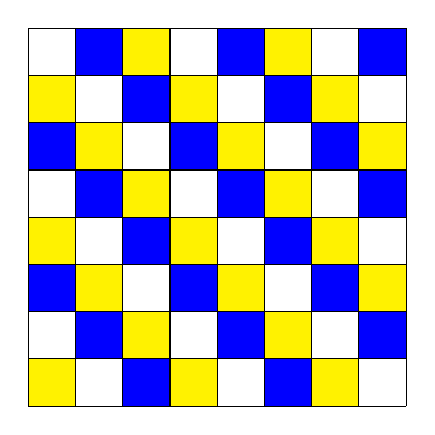
\begin{tikzpicture}[scale=0.6, baseline={(current bounding box.center)}]
\foreach \i in {0,...,7}{
  \foreach \j in {0,...,7}{
    \pgfmathparse{int(mod(\i+\j,3))}
    \ifnum\pgfmathresult=2
      \fill[color=blue] (\i,\j) rectangle (\i+1,\j+1);
    \fi
 
    \ifnum\pgfmathresult=0
      \fill[color=yellow] (\i,\j) rectangle (\i+1,\j+1);
    \fi
  }
}
\draw (0,0) grid (8,8);
\end{tikzpicture}

Offensichtlich hat man 22 weisse und 21 gelbe Felder, sowie 21 blaue und 21 rote Felder.
Wenn man nun einen $3\times 1$ Block umfärbt, färbt man immer einen gelben, einen blauen und einen weissen Block um. Um alle weissen Quadrate umzuformen braucht man eine gerade Anzahl $3\times 1$ Blöcke, für die blauen und gelben Blöcke braucht man eine ungerade Anzahl $3\times 1$ Blöcke. Dies ergibt einen Widerspruch. 
	

\textbf{Marking Scheme:}
\begin{itemize}
\item +1P: coloration avec 3 couleurs
\item +2P: compter deux types de cases avec un total différent, pair (22) et impair (21)
\item +1P: montrer qu'on doit utiliser un nombre \emph{pair} de coups
\item +2P: montrer qu'on doit utiliser un nombre \emph{impair} de coups
\end{itemize}


\newpage

%2
\item Seien $a$, $b$ und $c$ natürliche Zahlen. Finde den kleinsten Wert, den folgender Ausdruck annehmen kann:
\[
\frac{a}{\ggT (a+b,a-c)}+\frac{b}{\ggT (b+c,b-a)}+\frac{c}{\ggT (c+a,c-b)}.
\]


\textbf{1. Lösung (Paul):} 
Zuerst bemerken wir, dass 
\[
\ggT(a+b, a-c) = \ggT(a+b-(a-c), a-c) = \ggT(b+c, a-c) \leq b+c
\] gilt. Daraus folgt dann 
\[
\frac{a}{\ggT(a+b,a-c)}+\frac{b}{\ggT(b+c,b-a)}+\frac{c}{\ggT(c+a,c-b)} \geq \frac{a}{b+c}+\frac{b}{a+c}+\frac{c}{a+b} \geq \frac{3}{2},
\]
wobei die letzte Ungleichung Nesbitt ist. Durch einsetzen von $a=b=c$ sehen wir, dass $\frac{3}{2}$ tatsächlich erreicht werden kann.

\textbf{2. Lösung (Paul):}
Wir benutzen mehrmals, dass für $x,y \in \N$ gilt: $\ggT(x,y) \leq \min\{x,y\} \leq \max\{x,y\}$. Zuerst erledigen wir den Fall, dass mindestens zwei der Variablen gleich sind. OBdA wählen wir $a=b$. Gilt nun $a>c$, dann können wir den Ausdruck durch 
\[
\frac{a}{a-c} + \frac{a}{a + c} + \frac{c}{\ggT(a+c, c-a)} \geq 1 + \frac{1}{2} + 0 = \frac{3}{2}
\]
abschätzen. Im Fall $c>a$ schätzen wir den Ausdruck durch
\[
\frac{a}{a+b} + \frac{b}{b + c} + \frac{c}{c-b} \geq \frac{1}{2} + 0 + 1 = \frac{3}{2}
\]
ab. Bei $c=a$ gilt sogar Gleichheit zwischen allen Variabeln und der Ausdruck ist gleich $\frac{3}{2}$. Aufgrund der zyklischen Symmetrie genügt es, die Fälle $a>b>c$ und $a>c>b$ zu betrachten. Wir zeigen hier nur den ersten Fall. Ähnlich wie vorher können wir den Ausdruck durch
\[
\frac{a}{a-c} + \frac{b}{b+c} + \frac{c}{b-c} \geq 1 + \frac{b^2 + c^2}{b^2 - c^2} \geq 2 > \frac{3}{2}
\]
abschätzen. Insgesamt ist der Ausdruck also $\geq \frac{3}{2}$ und Gleichheit wird angenommen.


\textbf{Marking Scheme:}

\textbf{1. Lösung:}
\begin{itemize}
	\item 4P: Der Ausdruck ist $\geq \frac{a}{b+c}+\frac{b}{c+a} + \frac{c}{a+b}$
	\item 3P: Beweisen $\frac{a}{b+c}+\frac{b}{c+a} + \frac{c}{a+b} \geq \frac{3}{2}$
\end{itemize}
Im ersten Teil können folgende Teilpunkte gegeben werden:
\begin{itemize}
	\item 1P: $\ggT(a+b, a-c) = \ggT(a+b, b+c)$
	\item 1P: $\ggT(x, y) \leq x, y$ für $x, y>0$
\end{itemize}

\textbf{2. Lösung:}
In dieser Lösung sollen die Fälle $a=b>c$, $a>b=c$, $a>b>c$, $a>c>b$ und $a=b=c$ betrachten werden.
\begin{itemize}
	\item 1P: $\ggT(x, y)\leq \min(x, y) \leq x, y$ für $x, y>0$
	\item 1P: Fall $a=b>c$ durchlösen
	\item 1P: Fall $a>b=c$ durchlösen
	\item 2P: Einer der Fälle $a>b>c$ oder $a>c>b$ durchlösen
\end{itemize}
Oubli du cas d'égalité): -1P.



\newpage

%3
\item Finde alle natürlichen Zahlen $n$, für die kein Tripel natürlicher Zahlen $(a,b,c)$ existiert, sodass die folgende Gleichung erfüllt ist:
\[
n=\frac{a\cdot\kgV(b,c)+b\cdot\kgV(c,a)+c\cdot\kgV(a,b)}{\kgV(a,b,c)}.
\]


\textbf{Solution (Arnaud):} Les entiers $n$ recherchés sont les puissances de 2. On définit
\[
f(a,b,c):=\frac{a\cdot\kgV(b,c)+b\cdot\kgV(c,a)+c\cdot\kgV(a,b)}{\kgV(a,b,c)}.
\] 
Notons tout d'abord que 
\[
\frac{a\cdot\kgV(b,c)}{\kgV(a,b,c)}=\frac{a\cdot\kgV(b,c)}{\kgV(a,\ppcm(b,c))}=\gcd(a,\ppcm(b,c)).
\]
et donc 
\[
f(a,b,c)=\pgcd(a,\ppcm(b,c))+\pgcd(b,\ppcm(c,a))+\pgcd(c,\ppcm(a,b))\geq 3.
\]
Ainsi pour $n=1$ et $n=2$ il n'y a pas de solution $(a,b,c)$. De plus, $f$ est homogène de degré 1, i.e. $f(ka,kb,kc)=kf(a,b,c)$.

Supposons d'abord que $n\geq 3$ est impair. Si l'on cherche une solution avec $a=1$ et $b=c$ (pourquoi pas ?), alors on obtient 
\[
n=f\left(1,\frac{n-1}{2},\frac{n-1}{2}\right).
\]
Si $n=2^a\cdot n'$, avec $n'$ impair, alors par homogénéité on multiplie la solution pour $n'$ par $2^a$ pour obtenir une soltution pour $n$.

Supposons maintenant que $n=f(a,b,c)$ est une puissance de 2 et $n\geq 4$. Comme $n$ est pair, on doit avoir $a,b,c$ pairs. Si $a,b,c$ sont pairs, alors $n/2=f(a/2,b/2,c/2)$. Comme $n$ est une puissance de 2, $n/2$ est aussi une puissance de 2 et on peut répéter l'argument. On obtient après suffisamment d'itérations un triplet $(a',b',c')$ tel que $2=f(a',b',c')$. Ce qui est impossible.

\textbf{Marking Scheme:}

\underline{Cas $n=2^an'$}: 3P - avec points partiels:
\begin{itemize}
\item +1P: $f(ka,kb,kc)=kf(a,b,c)$,
\item +1P: construction pour $n\geq 3$ impair.
\end{itemize}

\underline{Cas $n=2^a$}: 4P - avec points partiels (max 3P):
\begin{itemize}
\item +1P: $f(a,b,c)\geq 3$,
\item +1P: exclure le cas "{au moins un impair}"
\item +2P: exclure le cas "{tous pairs}"
\end{itemize}


\newpage

%4
\item Sei $D$ ein Punkt im Inneren eines spitzwinkligen Dreiecks $ABC$, sodass $\angle BAD= \angle DBC$ und $\angle DAC=\angle BCD$. Sei $P$ ein Punkt auf dem Umkreis des Dreiecks $ADB$. Nehme an, $P$ befinde sich ausserhalb des Dreiecks $ABC$. Eine Gerade durch $P$ schneide den Strahl $BA$ in $X$ und den Strahl $CA$ in $Y$, sodass $\angle XPB=\angle PDB$ gilt. Zeige, dass sich $BY$ und $CX$ auf $AD$ schneiden.

\textbf{Lösung (Patrick):}
Durch die Aufgabenstellung ist gegeben, dass $\angle CAD = \angle DCB$. Mit dem Tangentenwinkelsatz erhält man, dass $BC$ eine Tangente zum Kreis $k_1$ durch $ADC$ und $k_2$ durch $ADB$ ist. Ebenso erhält man, dass $BC$ eine Tangente zu dem Umkreis von $ADB$ ist. Wir definieren $Z$ als den Schnittpunkt von $AD$ und $BC$. Des Weiteren definieren wir einen weiteren Punkt $U$, sodass $C,Z,B$ und $U$ in dieser Reiheinfolge auf der Gerade $BC$ liegen. Es gilt $\angle UBP = \angle BDP$. Es ist gegeben dass $\angle = BDP = \angle BPX$, somit findet man $\angle UBP = \angle BPX$, dass heisst die Geraden $BC$ und $PX$ sind parallel.
Mit dem Strahlensatz erhält man : $$\frac{AX}{XB}= \frac{AY}{YC}$$
Wenn man beweisen möchte, dass die Geraden $AZ, BY$ und $CX$ sich in einem Punkt schneiden, kann man Ceva verwenden. Somit muss man nur beweisen, dass : $$\frac{AX}{XB}\cdot\frac{YC}{AY}\cdot\frac{ZB}{CZ}=1$$
Da $Z$ auf der Potenzlinie zu $k_1$ und $k_2$ liegt, gilt $CZ = ZB$.
Das Einsetzen dieser Bedingung ergibt dann $$\frac{AX}{XB}\cdot\frac{YC}{AY}=1,$$
was schon durch den Strahlensatz bewiesen wurde.

	
\textbf{Marking Scheme:}
\begin{itemize}
\item $2 \times 1$P: zeigen, dass die Gerade $BC$ eine Tangente an die Kreise $ADB$ resp. $ADC$ ist.
\item 2P: feststellen, dass die Gerade $AD$ die Strecke $BC$ halbiert.
\item 1P: beweisen, dass $XP\parallel BC$ ist.
\item 1P: sinnvolle Verwendung des Strahlensatzes.
\item 1P: hilfreiche Verwendung von Ceva.
\end{itemize}

\newpage

%5
\item Zeige, dass keine Funktion $f\colon \R_{>0} \to \R_{>0}$ existiert, sodass für alle $x,y\in\R_{>0}$ gilt:
\[
f(xf(x)+yf(y))=xy.
\]

\textbf{Lösung (David):} Nehme an, $f$ sei eine Lösung der Gleichung.
Wir sehen zuerst, dass die rechte Seite alle möglichen Werte in $\R^+$ annehmen kann, also ist $f$ surjektiv. Dann existiert ein $c \in \R^+$ mit $f(c)=1/2$. Mit $x=y=c$ erhalten wir:
\[
f\left(c\cdot\frac{1}{2}+c\cdot\frac{1}{2}\right) = c^2 \quad \Longleftrightarrow \quad \frac{1}{2}=c^2 \quad \Longleftrightarrow \quad c=\frac{1}{\sqrt{2}}.
\] 
Insbesondere ist $f$ an diesem Punkt injektiv.
Mit $y=\frac{1}{\sqrt{2}}$ liefert uns die Gleichung 
\[ 
f\left(xf(x) + \frac{1}{2\sqrt{2}}\right) = \frac{x}{\sqrt{2}}.
\]
Da die rechte Seite noch immer jeden Wert in $\mathbb{R}^{+}$ annehmen kann, der Wert in der Klammer aber sicher grösser als $\frac{1}{2\sqrt{2}}$ ist, folgt, dass $f$ sogar surjektiv ist, wenn wir nur Werte $> \frac{1}{2\sqrt{2}}$ zulassen. Also finden wir für jedes $a \in \mathbb{R}^{+}$ ein $x > \frac{1}{2\sqrt{2}}$ mit $f(x) = 2\sqrt{2}\cdot a$. Dann gilt:
\[
xf(x) > \frac{1}{2\sqrt{2}} \cdot 2\sqrt{2}\cdot a = a
\]
Also kann $xf(x)$ beliebig grosse Werte annehmen. Mit $y=\frac{1}{2x}$ erhalten wir schlussendlich:
\[
f\left(xf(x) + \frac{1}{2x} f\left(\frac{1}{2x}\right)\right) = \frac{1}{2}
\]
Nun gilt einerseits aufgrund der Injektivität bei $1/2$, dass der Ausdruck in der Klammer $1/\sqrt{2}$ sein muss. Andererseits können wir $xf(x)$ und damit auch den ganzen Ausdruck in der Klammer beliebig gross machen. Widerspruch! Es kann somit keine solche Funktion geben.

\textbf{Lösung (Frieder):} 
On obtient de même 
\[
xf(x)+\frac{1}{2x}f\left(\frac{1}{2x}\right)=\frac{1}{\sqrt 2}.
\]
Donc $xf(x)<1/\sqrt 2$ pour tout $x$. Ainsi, avec $y=1$
\[
x=f(xf(x)+f(1))<\frac{1}{(xf(x)+f(1))\sqrt 2}<\frac{1}{f(1)}.
\]
Cette inégalité est vraie pour tout $x$. Contradiction.

\textbf{Marking Scheme:} 
\begin{itemize}
\item 2P: $f(a)=1/2\Rightarrow a=1/\sqrt 2$.
\item 1P: $xf(x)+\frac{1}{2x}f\left(\frac{1}{2x}\right)=1/\sqrt 2$.
\item 1P: $f((a,\infty))=\R^+$ pour $a>0$.
\item 1P: $xf(x)$ n'est pas borné.
\item 1P: $xf(x)<a$ pour $a>0$.
\end{itemize}




\newpage

%6
\item Sei $k$ der Inkreis des Dreiecks $ABC$ mit Inkreismittelpunkt $I$. Der Kreis $k$ berühre die Seiten $BC$, $CA$ und $AB$ in den Punkten $D$, $E$, respektive $F$. Sei $G$ der Schnittpunkt der Geraden $AI$ und des Kreises $k$, der zwischen $A$ und $I$ liegt. Nehme an, $BE$ und $FG$ seien parallel. Zeige, dass $BD=EF$ gilt.

\textbf{Lösung (Patrick):} 
Da $AI$ die Winkelhalbierende von $\angle CAB$ ist und $AE = AF$ gilt, sind die Dreiecke $AGE$ und $AGF$ kongruent. Somit gilt $\angle AEG = \angle AFG$. Da $AE = AF$, hat man auch $\angle AEF = \angle AFE$ und somit
      \[ \angle FEG = \angle FEA - \angle GEA = \angle FEG  = \angle AFE - \angle AFG = \angle EFG.  \]
Da $AE$ ist eine tangente zu $k$, gilt $\angle FEG= \angle FEG$.
Jetzt verwendet man die Tatsache, dass BE und FG parallel sind:
 \[   \angle FBE = \angle AFG = \angle GEF = \angle GFE  = \angle FEB. \]
Das heisst, dass $FE = BF$, und da $k$ der Inkreis von dem Dreieck $ABC$ ist, gilt $BD = BF$, womit man bewiesen hat, dass $BD = EF$.

\textbf{Marking Scheme:}
\begin{itemize}
\item 1P: $BF = BD$
\item 3P: Begründen, dass $\triangle AFG = \triangle AEG$
\begin{itemize}
	\item -1P: wenn man nur durch Symmetrie begründet ohne zusätzliche Angaben.
\end{itemize}
\item 1P: Tangentenwinkelsatz im Dreieck $\triangle EFG$
\item 1P: $FB = FE$ oder äquivalente Aussage
\end{itemize}


\newpage

%7
\item Sei $n$ eine natürliche Zahl. Sei $k$ die Anzahl Möglichkeiten, $n$ als Summe von einer oder mehreren aufeinanderfolgenden natürlichen Zahlen darzustellen. Zeige, dass $k$ der Anzahl ungerader positiver Teiler von $n$ entspricht.

\textbf{1. Lösung:}
Wir konstruieren zuerst für jeden ungeraden Teiler von $n$ eine Darstellung als Summe aufeinanderfolgender natürlicher Zahlen: \newline
Sei $a \in \N_0$ und $n = (2a+1) \cdot b$ für ein $b \in \N$. Betrachte die Nullsumme 
\[
(-a) + (-a+1) + \dots + (a-1) + a = 0.
\]
Addieren wir zu jedem der $2a+1$ Summanden $b$, (also insgesamt $(2a+1) \cdot b$ = n), erhalten wir
\[
(b-a) + (b-a+1) + \dots + (a+b-1) + (a+b) = n.
\]
Nun können allerdings noch nicht-positive Summanden auftreten, nämlich dann, wenn $a \geq b$ gilt. In diesem Fall können wir aber die Teilsumme
\[
(b-a) + \dots + (a-b) = 0
\]
einfach streichen und die Summe bleibt gleich, wobei die Anzahl der übrigen Summanden nun gerade ist. In beiden Fällen erhalten wir eine Summe aufeinanderfolgender natürlicher Zahlen mit Wert $n$, wie gewünscht. Wir müssen aber noch zeigen, dass die so konstruierten Summendarstellungen paarweise verschieden sind und es keine weiteren geben kann.
\newline
Für die erste Aussage betrachten wir eine konstruierte Summe. Da der grösste Summand $s_{max}$ durch $(a+b)$ und der kleinste Summand $s_{min}$ durch $(b-a)$ (ungerade Anzahl Summanden), respektive $(a-b+1)$ (gerade Anzahl Summanden) gegeben ist, können wir $a$ und $b$ direkt anhand von $s_{min}$, $s_{max}$ und der Anzahl Summanden bestimmen. Also sind für verschiedene $(a,b)$ auch die konstruierten Summen verschieden.
\newline
Betrachte nun beliebige Summe aufeinanderfolgender Zahlen mit Wert $n$. Besteht diese aus einer geraden Anzahl Summanden, können wir sie durch Addition von
\[
(-s_{min}+1) + \dots + (s_{min}-1)
\]
zu einer Summe mit ungerader Anzahl Summanden machen. Dann können wir sie durch Subtraktion ihres arithmetischen Mittels (das bei einer ungeraden Anzahl aufeinanderfolgenden Zahlen dem Median entspricht, also insbesondere ganzzahlig ist!) von jedem Summand zu einer Nullsumme machen. Da der so subtrahierte Wert einerseits sicher durch die Anzahl Summanden teilbar ist und andererseits $n$ beträgt, folgt, dass die Anzahl Summanden der 'Endsumme' ein Teiler von $n$ ist. Also gibt es keine weiteren Summen als die, die wir im ersten Teil konstruiert haben. Es sind also genau $k$.

\textbf{2. Lösung:} On considère les sommes 
\[
	n = x + (x+1) + \ldots + (x + k-1) = kx + \frac{k(k-1)}{2}
\]
avec $x, k\in \N$. On obtient donc la formule
\[
	n = \left\{\begin{array}{ll}
	k(x+\frac{k-1}{2}) & \mbox{si } k \mbox{ est impair.}\\
	\frac{k}{2}(2x+k-1) & \mbox{si } k \mbox{ est pair.}
	\end{array}\right.
\]

Arrivés à ce point, on devine que si $k$ est impair, le diviseur impair associé à la somme est $k$, est que si $k$ est pair ce diviseur est $2x+k-1$. On a ainsi réussi à associer à chaque somme un unique diviseur impair de $n$. Si on arrive à montrer que chaque diviseur impair de $n$ est associé à une certaine somme et que à deux sommes différentes sont associés deux diviseurs impairs différents on aura donc terminé l'exercice.

Pour cela prenons un diviseur impair $d$. Le diviseur $d$ est associé à une somme avec $k$ impair si il existe des entiers naturels $k$, $x$ tels que
\[
	k = d \quad \mbox{et}\qquad x + \frac{k-1}{2} = \frac{n}{d}.
\]
Pour cela il faut que $x = \frac{n}{d} - \frac{k-1}{2} = \frac{n}{d} - \frac{d-1}{2}$, donc on peut associer $d$ à une somme avec $k$ impair si et seulement si $\frac{n}{d} > \frac{d-1}{2}$ et dans ce cas il est associé à une unique telle somme. Le diviseur $d$ est associé à une somme avec $k$ pair si il existe des entiers naturels $k$, $x$ tels que
\[
	\frac{k}{2} = \frac{n}{d} \qquad \mbox{et} \quad 2x + k - 1 = d.
\]
Pour cela il faut que $x = \frac{d+1}{2} - \frac{k}{2} = \frac{d+1}{2} - \frac{n}{d}$, donc on peut associer $d$ à une somme avec $k$ pair si et seulement si $\frac{n}{d} < \frac{d+1}{2}$ et dans ce cas il est associé à une unique telle somme.

Puisque pour tout diviseur impair $d$, parmi les conditions $\frac{n}{d} > \frac{d-1}{2}$ et $\frac{n}{d} < \frac{d+1}{2}$ exactement une des deux est vraie, chaque diviseur impair est associé à exactement une somme, ce qui conclut l'exercice.



\textbf{Marking Scheme:}
\begin{itemize}
	\item 2P: Konstruktion von Summen mit ungerader Anzahl Summanden aus einem Teiler.
	\item 2P: Konstruktion von Summen mit gerader Anzahl Summanden aus einem Teiler.
	\item +1P: Alle konstruierte Summen sind unterschiedlich.
	\item +1P: Alle Summen werden konstruiert.
\end{itemize}
Bei unvollständigen Lösungen ergeben die zwei letzte Schritte höchstens einen Punkt.


\newpage

%8
\item Seien $a$, $b$, $c$, $d$ und $e$ positive reelle Zahlen. Bestimme den grössten Wert, den folgender Ausdruck annehmen kann:
\[
\frac{ab+bc+cd+de}{2a^2+b^2+2c^2+d^2+2e^2}.
\]


\textbf{Solution (Arnaud):} L'idée est clairement d'appliquer AM-GM. On doit donc décomposer $b^2=xb^2+yb^2$ et probablement $2c^2=c^2+c^2$. Les nombres $x,y$ doivent donc satisfaire $x+y=1$ et $2x=y$. On obtient $x=1/3$ et $y=2/3$. Par AM-GM, on obtient
\begin{align*}
2a^2+1/3b^2&\geq 2\sqrt{2/3}\cdot ab,\\
2/3b^2+c^2&\geq 2\sqrt{2/3}\cdot bc,\\
c^2+2/3d^2&\geq 2\sqrt{2/3}\cdot cd,\\
1/3d^2+2e^2&\geq 2\sqrt{2/3}\cdot ed.\\
\end{align*}
Le maximum est donc $(2\sqrt{2/3})^{-1}=\sqrt{3/8}$. Les cas d'égalité sont donnés par les applications d'AM-GM. On obtient par exemple $a=1,b=\sqrt{6},c=2,d=\sqrt{6}$ et $e=1$.

\textbf{Marking Scheme:}
\underline{L'expression ne dépasse pas $\sqrt{\frac{3}{8}}$:} : 5P.
\begin{itemize}
	\item 0P: Séparer le dénominateur comme $(2a^+b^2+c^2) + (c^2+d^2+2e^2)$
	\item 1P: Essayer d'appliquer AM-GM après avoir séparé le dénominateur.
\end{itemize}
\underline{L'expression atteint $\sqrt{\frac{3}{8}}$} : 2P.


\newpage

%9
\item Sei $n$ eine natürliche Zahl und $G$ die Menge der Punkte $(x,y)$ in der Ebene, sodass $x$ und $y$ ganze Zahlen mit $1\leq x,y \leq n$ sind. Eine Teilmenge von $G$ heisst \textit{parallelogrammfrei}, wenn sie keine vier nicht-kollineare Punkte enthält, die die Eckpunkte eines Parallelogramms sind. Wie viele Elemente kann eine parallelogrammfreie Teilmenge von $G$ höchstens enthalten?

\textbf{Lösung (Cyril):}
Die maximal Anzahl Elemente ist $2n-1$. 

\begin{itemize}
\item \textbf{$\geq 2n-1$}: Wir nehmen alle Punkte der Form $(0,y)$ und $(x,0)$. Wenn wir nun 4 Punkte wählen, sind mindestens drei davon kollinear und können daher kein Parallelogramm bilden.
\item \textbf{$\leq 2n-1$}: Wir beweisen, dass wenn wir $2n$ Punkte wählen, dass wir dann ein Parallelogramm finden, bei dem jeweils 2 Punkte die gleiche $x$-Koordinate haben. (wir beweisen also etwas leicht Stärkeres).

Nehme dafür an, wir können $2n$ Punkte wählen, ohne ein solchen Parallelogramm zu bilden. Wir fügen diese Punkte nun nacheinander zu unserer Menge hinzu, wobei wir dies in Reihenfolge aufsteigender $y$-Koordinate machen. 

Für jeden Punkt den wir zu der Menge hinfügen, betrachten wir die Distanz zum Punkt mit der kleinsten $y$-Koordinate und gleicher $x$-Koordinate. Sobald wir zweimal die gleiche strikt positive Distanz antreffen, müssen die entsprechenden Punkte ein Parallelogramm bilden (da diese nicht alle die gleiche $x$-Koordinate haben können, da wir jeweils die Distanz zur kleinsten $y$-Koordinate nehmen).

Wir können nun fast mit Schubfach fertig machen. Wir müssen nur noch sehen, dass die möglichen Distanzen von 0 bis $n-1$ gehen (0, falls es der Punkt mit der kleinsten $y$-Koordinate ist) und wir maximal $n$ Punkte mit Distanz 0 haben. Daher müssen wir zweimal de gleiche Distanz haben, die nicht 0 ist.
\end{itemize}

\textbf{Marking Scheme:}
\begin{itemize}
	\item 1P: Idee, Schubfachprinzip mit vektoriellen Distanzen als Perlen zu verwenden
	\item 2P: Reduktion des Problems auf horizontale/vertikale Distanzen
	\item 2P: Zählen, wie viele Distanzen innerhalb einer 'Zeile' oder 'Spalte' auftreten
	\item 2P: Konstruktion einer parallelogrammfreien Menge mit $2n-1$ Punkten
\end{itemize}


\newpage

%10
\item Sei $p\geq 2$ eine Primzahl. Louis und Arnaud wählen abwechselnd einen Index $i\in\{0,1,\ldots,p-1\}$, der bisher noch nicht gewählt wurde, und eine Ziffer $a_i\in\{0,1,\ldots,9\}$. Louis beginnt. Wenn alle Indizes ausgewählt wurden, berechnen sie die folgende Summe:
\[
a_0+a_1\cdot 10+\ldots+a_{p-1}\cdot 10^{p-1}=\sum_{i=0}^{p-1}a_i\cdot 10^i.
\]
Wenn diese Summe durch $p$ teilbar ist, gewinnt Louis, ansonsten gewinnt Arnaud. Zeige, dass Louis eine Gewinnstrategie hat.

\textbf{Solution:}
Wir sagen, dass ein Speiler den Zug $(i, a_i)$ spielt, wenn er in diesem Zug den Index $i$ und die Ziffer $a_i$ gewählt hat.

Wenn $p=2$ oder $p=5$, dann macht Louis als erstes den Zug $(0,0)$ und gewinnt, da die Summe ein Vielfaches von $10$ sein wird.

Nehme nun an, dass $p$ weder $2$ noch $5$ ist. Louis wählt nun als ersten Zug $(p-1,0)$. Mit Fermat gilt $(10^{(p-1)/2})^2=10^{p-1}\equiv 1 \mod{p}$., also $p\mid (10^{(p-1)/2})^2-1=(10^{(p-1)/2}-1)(10^{(p-1)/2}+1)$. Weil $p$ prim ist, gilt somit $p\mid (10^{(p-1)/2}-1)$ oder $p\mid (10^{(p-1)/2}-1)$. Wir haben also folgende zwei Fälle:

Fall 1: $10^{(p-1)/2}\equiv -1\mod p$

Wenn nun Arnaud den Zug $(i, a_i)$ macht, macht Louis den Zug $(j,a_j)=(i+\frac{p-1}{2},a_i)$ für $0\leq i\leq \frac{p-3}{2}$, beziehungsweise den Zug $(j,a_j)=(i-\frac{p-1}{2},a_i)$ für $\frac{p-1}{2}\leq i\leq p-2$. Bemerke, dass Louis immer einen solchen Zug machen kann: Vor einem Zug von Arnaud wurden von jeder Menge der Form $\{r, r+(p-1)/2\}$ entweder beide Elemente oder kein Element schon bei vorherigen Zügen als Indices ausgewählt. Somit ist nach jedem der Züge von Louis die Summe der bisher ausgewählten Paare durch $p$ teilbar, und damit gewinnt Louis.

Fall 2: $10^{(p-1)/2}\equiv 1\mod p$

Wenn nun Arnaud den Zug $(i, a_i)$ macht, macht Louis den Zug $(j,a_j)=(i+\frac{p-1}{2},9-a_i)$ für $0\leq i\leq \frac{p-3}{2}$, beziehungsweise den Zug $(j,a_j)=(i-\frac{p-1}{2},9-a_i)$ für $\frac{p-1}{2}\leq i\leq p-2$. Wie oben folgt, dass Louis immer so einen Zug machen kann. Wir haben $10^j\equiv 10^i\mod p$, und somit gilt $a_j\cdot 10^j+a_i\cdot 10^i\equiv (a_i+a_j)\cdot 10^i=9\cdot 10^i\mod p$. Also wird am Schluss des Spiels die Summe aller Terme kongruent zu 
\[ \sum_{i=0}^{\frac{p-3}{2}}9\cdot 10^i=10^{(p-1)/2}-1\equiv 0\mod p \]
und somit gewinnt Louis.

\textbf{Marking Scheme:}
\begin{itemize}
	\item 1P: $10^{\frac{p-1}{2}} \equiv \pm 1 \mod(p)$.
	\item 2P: Prouver dans le cas $10^{\frac{p-1}{2}} \equiv 1 \mod(p)$.
	\item 4P: Prouver dans le cas $10^{\frac{p-1}{2}} \equiv -1 \mod(p)$.
\end{itemize}

\end{enumerate}


\bigskip

\vspace{1cm}

\end{document}
